%%%%%%%%%%%%%%%%%%%%%%%%%%%%%%%%%%%%%%%%%%%%%%%%%%%%%%%%%%%%%%%%%%%%%%%%%%%%
%%                                                                        %%
%%                 Support de cours Programmation orientée objet                  %%
%%                                                                        %%
%%%%%%%%%%%%%%%%%%%%%%%%%%%%%%%%%%%%%%%%%%%%%%%%%%%%%%%%%%%%%%%%%%%%%%%%%%%%
%% Guillaume Moreau (EC Nantes)
%% création : 21/06/2004
%% dernière modification : 23/06/2004
%% historique :

%% il faut fixer l'URL base pour que les liens relatifs fonctionnent...
%% bizaremment fichu mais c'est comme ça.

\documentclass[allowframebreaks,xcolor=dvipsnames]{beamer}

\mode<presentation>
{
\usetheme{Antibes}
  % or ...

  %\setbeamercovered{transparent}
  % or whatever (possibly just delete it)
}
\useoutertheme{infolines}
\usecolortheme[named=RoyalBlue]{structure}

\uselanguage{french}
\languagepath{french}
\deftranslation[to=french]{definition}{définition}
\deftranslation[to=french]{Definition}{D\'efinition}

\setbeamertemplate{blocks}[rounded][shadow=true]
\setbeamertemplate{navigation symbols}{}
\setbeamertemplate{itemize item}[square]
\setbeamertemplate{itemize subitem}[triangle]

\usepackage[T1]{fontenc}
\usepackage[utf8]{inputenc}
% or whatever

\usepackage[french]{babel}
% or whatever

%% pour afficher le plan à chaque début de section
%\AtBeginSection[]{
%  \begin{frame}{Plan}
%  \tiny \tableofcontents[currentsection, hideothersubsections]
%  \end{frame}
%}


%% tout ce qui est relatifs aux extraits de code
\usepackage{listings}
\usepackage{lstautogobble}
\lstloadlanguages{C++}
\lstset{% paramètres généraux des listings
	language=C++,
	basicstyle=\ttfamily\tiny, %% style général : chasse fixe, taille minimale
	keywordstyle=\color{webgreen}\bfseries, % les mots clés en vert et gras
	stringstyle=\color{blue}, % les chaines de caractères en bleu
	commentstyle=\color{webbrown},
	autogobble
}


\usepackage{myslides}

%\usepackage{times}
\usepackage[T1]{fontenc}
% Or whatever. Note that the encoding and the font should match. If T1
% does not look nice, try deleting the line with the fontenc.


\title[Option RV / CPLUS] % (optional, use only with long paper titles)
{Programmation C++}

\author[G. Moreau]{Guillaume Moreau\\
\texttt{guillaume.moreau@ec-nantes.fr}}
% - Use the \inst{?} command only if the authors have different
%   affiliation.

\institute[Ecole Centrale de Nantes] % (optional, but mostly needed)
{
  Ecole Centrale de Nantes
}

\date % (optional)
{Septembre 2015}

\subject{Cours Programmation C++}


\definecolor{webgreen}{rgb}{0,.5,0}
\definecolor{webbrown}{rgb}{.6,0,0}
\definecolor{* }{rgb}{0,.5,0}
\definecolor{. }{rgb}{.6,0,0}

% option d'affiche de table des matières : http://mirror.unl.edu/ctan/macros/latex/contrib/beamer/doc/beameruserguide.pdf
% section 10.5

% Delete this, if you do not want the table of contents to pop up at
% the beginning of each subsection:
\AtBeginSection[]
{
   \begin{frame}
       \frametitle{Plan}
       \tableofcontents[sectionstyle=show/hide,subsectionstyle=show/show/hide,subsubsectionstyle=hide/hide]
   \end{frame}
}

\AtBeginSubsection[]
{
	\begin{frame}
		\frametitle{Plan}
		\tableofcontents[sectionstyle=show/hide,subsectionstyle=show/shaded/hide,subsubsectionstyle=show/show/hide]
	\end{frame}
}

\begin{document}

\begin{frame}
  \titlepage
\end{frame}

\begin{frame}[allowframebreaks]{Plan du cours}
  \tableofcontents[hideallsubsections]
  % You might wish to add the option [pausesections]
\end{frame}


\section{Introduction}

% introduction au cours de C++

\subsection{Pourquoi C++ dans l'option RV ?}

\begin{frame}{Qu'est-ce que C++ ?}
\begin{figure}[htbp]
\begin{center}
   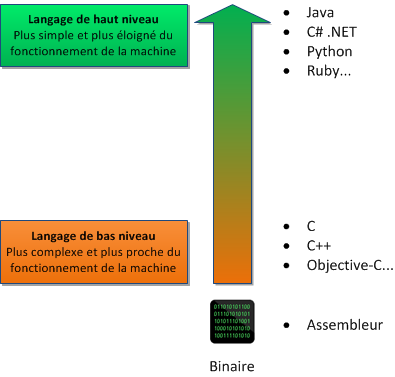
\includegraphics[scale=0.6]{fig/langages.png}
   \caption{(c) OpenClassrooms}
\end{center}
\end{figure}
\end{frame}

\subsection{Historique}

\begin{frame}{Histoire}
\begin{itemize}
\item 1958 : Algol
\item années 60 : CPL, puis BPCL puis B
\item 1970 : langage C (Dennis Ritchie 1969-1973)
\item 1979 : \textit{C with classes}
\item 1983 : C++ (amélioration du C ) : Bjarne Stroustrup
\item 1989 : C++ 2.0 (héritage multiple, classes abstraites)
\item 1995 : java
\item 1998 : début de la normalisation de C++ (inclusion de la \textit{SL})
\item 2011 : \textbf{C++11 devient un standard ISO}
\item 2014 : nouvelle norme C++14
\item 2017 : c++17 : définition figée en avril 2017, acceptation ISO/ANSI
\item 2020 : c++20 : en retard
\end{itemize}
\end{frame}

\begin{frame}[fragile]
   \frametitle{C à l'ancienne}
   \begin{itemize}
      \item Pour mémoire, C est un langage qui permet des choses un peu \emph{roots}
   \end{itemize}
   \pause 
   \begin{lstlisting}
      int a;
      a = a+++++a; // forbidden since C89
   \end{lstlisting}
   \pause
   \begin{lstlisting}
      switch(0)
      i++;
   \end{lstlisting}
   \pause 
   \begin{lstlisting}
      #define boo() 123
      #define foo(y) boo y )
      #define open (
      foo(open)
   \end{lstlisting}
   \pause
   \begin{lstlisting}
      #include<stdio.h>
      int main(){int a=0,b=a;long long c[178819],d=8,e=257,f,g,
      h,i=d-9;for(;a<178819;){c[a++]=i;}for(a*=53;a;a>>=8)putc\
      har(a);if((f=getchar())<0)return 0;for(;(g=getchar())>=0;
      ){h=i=g<<8^f;g+=f<<8;a=e<(512<<a%8|(a<7))||f>256?a:a>6?15
      :a+1;for(;c[i]>-1&&c[i]>>16!=g;)i+=i+h<69000?h+1:h-69000;
      h=c[i]<0;b|=h*f<<d;for(d+=h*(a%8+9);d>15;d-=8)putchar(b=b
      >>8);f=h?g-f*256:c[i]%65536L;if(a<8*h){c[i]=g*65536L|e++;
      }}b|=f<<d;for(d+=a%8;d>-1;d-=8)putchar(b>>=8);return!53;}
   \end{lstlisting}
\end{frame}

\subsection{Organisation du cours}

\begin{frame}{Organisation}
\begin{itemize}
\item Peu de cours, beaucoup de pratique
\item un DS sur table à la fin (évaluation individuelle)
\item Base de travail
\begin{itemize}
\item Norme "C++11-14"
\item Utilisation de la machine virtuelle Linux installée en B114
\item outils : make, gcc
\item IDE ou éditeurs de texte : à votre convenance
\begin{alertblock}{Avertissement}
Vous pouvez utiliser d'autres outils (compilateurs), mais à vos risques et périls !
\end{alertblock}
\end{itemize}
\end{itemize}
\end{frame}

\begin{frame}{A propos des TP}
   \begin{itemize}
      \item Tous les TP rendus sont corrigés 
      \item Aucun TP n'est noté 
      \item En clair
      \begin{itemize}
         \item Chacun travaille à son rythme
         \item Cela ne sert à rien de rendre le TP du voisin parce qu'on est en retard
         \item Lire le C++ $\neq$ écrire le C++ 
         \item On ne peut pas rendre les TP, mais cela consiste à aller au DS sans filet
      \end{itemize}
   \end{itemize}
\end{frame}

\section{Rappels rapides}

% % rappels sur ce qui a été vu en ALGPR
\subsection{Vos (anciens) premiers pas en C++}

\begin{frame}[fragile]
\frametitle{Premier programme C++}
\begin{lstlisting}[language=C++]
#include <iostream>
using namespace std;

/* fonction principale du programme

	Elle affiche un message
*/
int main() {
  cout << "hello world" << endl;

  return 0;
}
\end{lstlisting}
\end{frame}

\begin{frame}{Ligne par ligne}
\begin{itemize}
\item \texttt{\#include <iostream>} : inclure des fichiers de \textbf{déclaration} d'autres fonctions
\item \texttt{using namespace std;}: utiliser un espace de nommage, plus tard !
\item \texttt{/* ... */} définit une zone de commentaires (pas interprétée par le compilateur)
\item \texttt{int main() $\{$ ... $\}$} : fonction principale, appelée au lancement du programme
\item \texttt{cout << "hello world" << endl;} : façon \textit{moderne} d'afficher du texte
\item \texttt{return 0;} : la fonction \textit{main()} est supposée retourner un entier
\end{itemize}
\end{frame}

\begin{frame}[fragile]
\frametitle{Compilation et édition des liens (v1)}
\begin{itemize}
\item Compilation : transformation d'un fichier source en code \textit{objet}
\item Edition des liens : assemblage de plusieurs fichiers objet pour en faire un exécutable (\texttt{.exe} sous Windows, pas d'extension obligatoire sur les autres systèmes)
\end{itemize}
\pause \begin{block}{En ligne de commande}
\begin{verbatim}
g++ -c premierprog.cxx
g++ -o premierprog.out premierprog.o
\end{verbatim}
\end{block}

\pause \begin{exampleblock}{Exécution}
\begin{verbatim}
./premierprog.out
hello world
\end{verbatim}
\end{exampleblock}
\end{frame}

% tous sur les makefiles
\subsection{Makefiles}

\begin{frame}{Motivations}
  \begin{itemize}
  \item Gérer plusieurs fichiers source et l'ensemble du processus de compilation / éditions des liens en une seule opération
  \begin{itemize}
  \item Faire plus ou moins l'équivalent des IDE comme Visual Studio
	\begin{itemize}
		\item Note : il y a moins bien (\texttt{make}), mais il y a aussi beaucoup mieux...
		\item VS ne sait pas gérer le multi-plateformes (et pour cause)
		\item VS ne sait pas trouver vos bibliothèques tout seul
	\end{itemize}
  \item Pour un gros projet : ne recompiler que le strict minimum nécessaire
  \end{itemize}
  \item Rappels : différentes phases
  \begin{itemize}
  \item Compilation des fichiers source (on a encouragé leur multiplication !)
  \item Edition des liens
  \end{itemize}

  \end{itemize}
\end{frame}

\begin{frame}{Principe}
  \begin{itemize}
  \item 2 étapes
  \begin{itemize}
  \item Ecriture d'un fichier \texttt{Makefile} (modifé à chaque fois qu'on ajoute un nouveau fichier source
  \item Compilation/Edition des liens : appel de la commande \texttt{make}
  \end{itemize}
  \begin{exampleblock}{Exemple}
  	Soit un programme exécutable \texttt{machin.out} construit à partir de 3 fichiers source \texttt{main.cxx}, \texttt{f1.cxx} et \texttt{f2.cxx}. Construction :
  	\begin{itemize}
  		\item \texttt{g++ -c main.cxx}
  		\item \texttt{g++ -c f1.cxx}
  		\item \texttt{g++ -c f2.cxx}
  		\item \texttt{g++ -o machin.out main.o f1.o f2.o}
  	\end{itemize}
  \end{exampleblock}
  \end{itemize}
\end{frame}

\begin{frame}{Graphe de dépendances}
  \begin{itemize}
  \item Ecrire quel fichier dépend de quel autre
  \begin{itemize}
  \item \texttt{machin.out} dépend de \texttt{main.o}, \texttt{f1.o} et \texttt{f2.o}
  \item \texttt{main.o} dépend de \texttt{main.cxx}
  \item \texttt{f1.o} dépend de \texttt{f1.cxx}
  \item \texttt{f2.o} dépend de \texttt{f2.cxx}
  \end{itemize}
  \item Les règles permettant de reconstruire les fichiers .out et .o sont connues
  \end{itemize}
      \begin{center}
      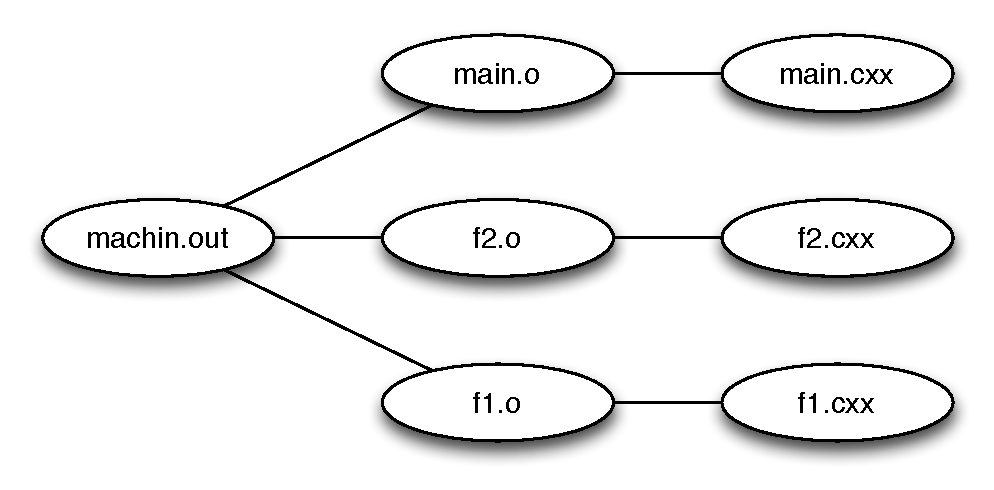
\includegraphics[scale=.43]{fig/base-dependance.pdf}
    \end{center}

\end{frame}

\begin{frame}{Dépendance temporelle}
  \begin{itemize}
  \item La date et l'heure du fichier sont utilisées : un fichier doit toujours être plus récent que les fichiers à sa droite dont il dépend
  \item Si ce n'est pas le cas, l'opération de production du fichier de gauche est lancée
  \item Le processus est itéré jusqu'à ce que toutes les règles soient respectées
  \end{itemize}
\end{frame}

\begin{frame}{Exemple (1/3)}
        \begin{center}
      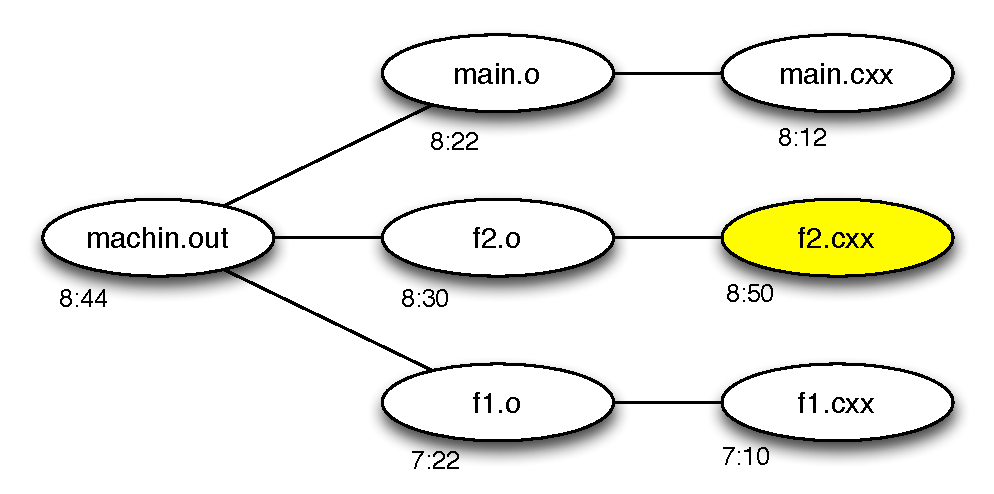
\includegraphics[scale=.6]{fig/base-dependance1.pdf}
    \end{center}
\end{frame}

\begin{frame}{Exemple (2/3)}
        \begin{center}
      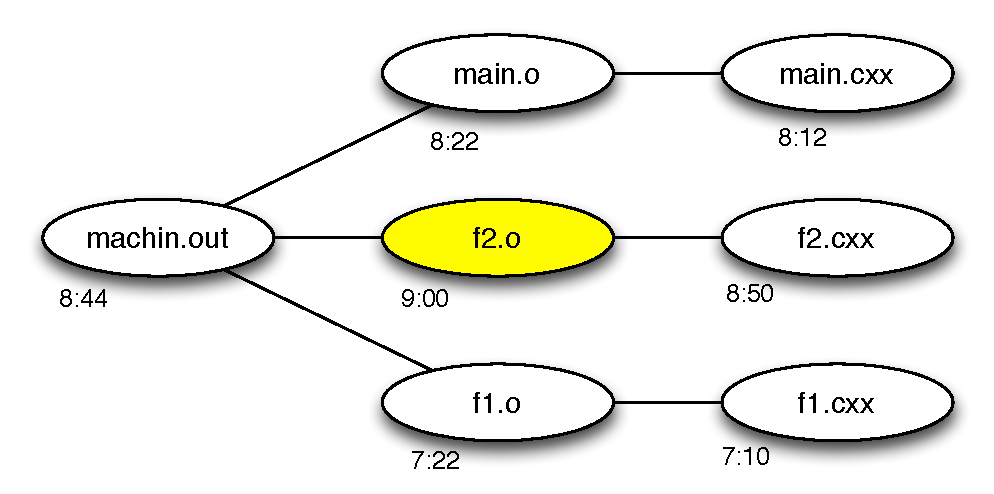
\includegraphics[scale=.6]{fig/base-dependance2.pdf}
    \end{center}
\end{frame}

\begin{frame}{Exemple (3/3)}
        \begin{center}
      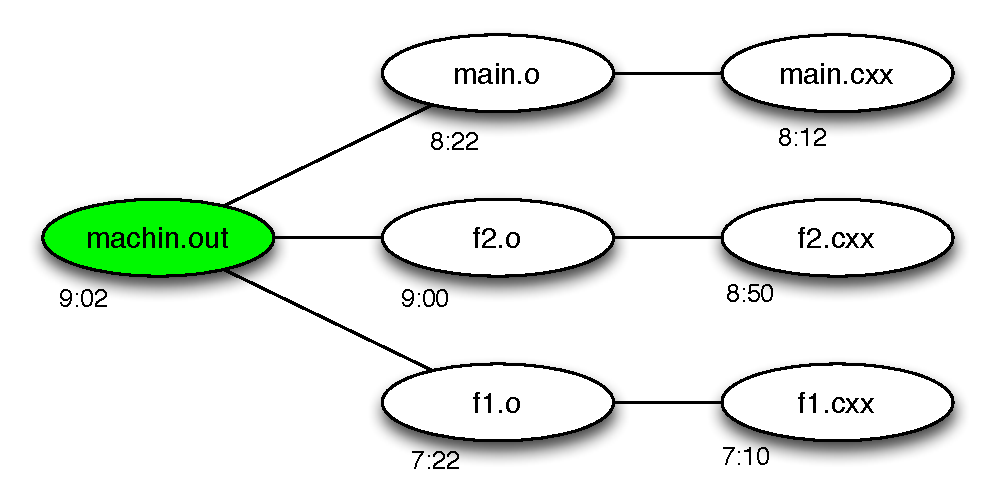
\includegraphics[scale=.6]{fig/base-dependance3.pdf}
    \end{center}
\end{frame}

\begin{frame}{Syntaxe du \texttt{Makefile}}
\begin{block}{Ensemble de règles de la forme}
\texttt{  fichier: fichier1 fichier2 fichier3 ... \\
  	<TAB>régle de production de fichier \\
}\end{block}
\begin{itemize}
\item Note : le fichier s'appelle obligatoirement \texttt{Makefile}
\begin{itemize}
\item Sauf parfois sous Windows, qui n'aime pas les fichiers sans extensions...
\end{itemize}
\item La première règle est toujours celle qui produit l'exécutable
\begin{itemize}
	\item en fait non, c'est juste celle qui sera vérifiée en premier par \texttt{make}
\end{itemize}
\item Ensuite il suffit d'appeler la commande \texttt{make}
\end{itemize}
\end{frame}

\begin{frame}[fragile]
  \frametitle{Makefile de l'exemple}
        \begin{center}
      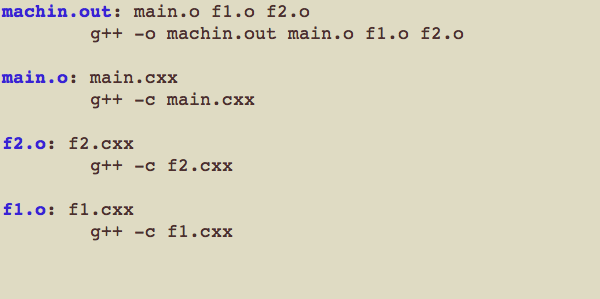
\includegraphics[scale=.4]{fig/makefile.png}
    \end{center}
\end{frame}


\subsection{Syntaxe générale du langage C(++)}

\begin{frame}[fragile]
\frametitle{Commentaires}
\begin{lstlisting}[language=C++]
/* Ceci est un commentaire qui peut etre long */

// Ceci est un commentaire d'une ligne
\end{lstlisting}
\begin{itemize}
\item nécessaires (mais pas suffisants) à se remettre dans le code 6 mois plus tard
\item nécessaires (mais pas suffisants) pour donner son code à quelqu'un d'autre
\item Éléments de qualité du code (métriques)
\end{itemize}

\end{frame}


\begin{frame}[fragile]
\frametitle{Types de base en C(++)}
\begin{itemize}
\item Entiers
\begin{itemize}
\item caractères : \verb|char| (entiers sur 8 (?) bits)
\item entiers classiques : \verb|int|, \verb|short| (16 bits), \verb|long| (32 bits), \verb|long long| (64 bits)
\item utilisation possible des préfixes \verb|signed| et \verb|unsigned|
\item il existe aussi des types de taille fixe : \verb|int8_t|, \verb|uint8_t|,... définis dans \verb|stdint.h|
\end{itemize}
\item types flottants
\begin{itemize}
\item simple précision : \verb|float|
\item double précision : \verb|double|
\end{itemize}
\item Les constantes sont préfixées par \verb|const|
\end{itemize}
\end{frame}

\begin{frame}[fragile]
\frametitle{Enregistrements}
\begin{itemize}
\item Définition d'un enregistrement
\begin{lstlisting}
struct nomtype {
	type1 attribut1;
	...
	typeN attributN;
};
\end{lstlisting}
\begin{codeblock}{Exemple}
\begin{lstlisting}
struct complexe {
	float re,im;
};
\end{lstlisting}
\end{codeblock}
\item Déclaration d'une variable de type enregistrement : \verb|nomtype nomvar;|
\item Accès aux attributs : \verb|nomvar.attributI|
\item La comparaison directe \verb|==| n'est pas possible, mais la copie (superficielle) est possible avec \verb|=|
\end{itemize}
\end{frame}

\begin{frame}[fragile]
\frametitle{Blocs d'instructions}
\begin{itemize}
\item instruction simple \verb|<I> : I;|
\item Bloc d'instructions \verb|<B> : { I1; ... IN; }|
\item En C, les déclarations de variables doivent se faire en \textbf{début de bloc}. En C++, on peut les faire n'importe où, mais ce n'est pas recommandé pour autant
\item Portée des variables : bloc d'instructions dans lequel elles sont déclarées
\end{itemize}
\end{frame}

\begin{frame}[fragile]
\frametitle{Opérateurs}
\begin{itemize}
\item Affectation : \verb|=|
\item Arithmétique :
\begin{itemize}
\item addition : \verb|+|
\item soustraction : \verb|-|
\item multiplication : \verb|*|
\item division : \verb|/|
\item modulo : \verb| %|
\end{itemize}
\item Opérateurs raccourcis : \verb|+=,-=,*=,/=|...
\item Incrémentation, décrémentation : \verb|++| et \verb|--| sous forme préfixe ou suffixe
\item Opérations sur les bits :
\begin{itemize}
\item \verb#&,|,^# : et, ou, ou exclusif
\item décalages bit à bit : \verb|<<| et \verb|>>|
\end{itemize}
\item Opérateur ternaire \verb|(| \textit{condition} \verb|?| \textit{action1} \verb|:| \textit{action2} \verb|)|
\end{itemize}
\end{frame}

\begin{frame}[fragile]
\frametitle{Structures de contrôle}
\begin{itemize}
\item Syntaxe 1 : \verb|if (|\textit{condition}\verb|)| \textit{bloc1}
\item Syntaxe 2 : \verb|if (|\textit{condition}\verb|)| \textit{bloc1} \verb|else| \textit{bloc2}
\item \alert{Attention} : les parenthèses autour de la condition sont obligatoires
\item \textit{condition} est une expression de type booléen (\verb|int| en C à l'ancienne qui n'a pas de type de booléen)
\begin{itemize}
\item 0 pour faux, n'importe quelle autre valeur est vraie
\end{itemize}
\item Opérateurs pour les expressions booléennes
\begin{itemize}
\item \verb|&&|, \verb#||#, \verb|!|, \verb|==|, \verb|!=|
\item ainsi évidemment que \verb|<|, \verb|<=|, \verb|>=|, \verb|>|
\end{itemize}
\item Opérateur de sélection : \verb|switch(|\textit{var-num}\verb|) {| \textit{liste de cas} \verb|}|
\begin{itemize}
\item cas : \verb|case |\textit{nombre}\verb|:| \textit{liste d'instructions} \verb|break;|
\item cas par défaut (en dernier) : \verb|default:|  \textit{liste d'instructions}
\end{itemize}
\end{itemize}
\end{frame}

\begin{frame}[fragile]
\frametitle{Structures itératives}
\begin{itemize}
\item \verb|while (|\textit{condition}\verb|) {| \textit{liste d'instructions} \verb|}| : répète la liste d'instructions tant que la condition \textit{condition} est vraie
\begin{itemize}
\item La condition est évaluée \structure{avant} chaque exécution de la liste d'instructions
\end{itemize}
\item \verb|for (|\textit{initialisation} \verb|;| \textit{invariant} \verb|;| \textit{incrément} \verb|) {| \textit{liste d'instructions} \verb|}|
\begin{itemize}
\item La liste d'instructions est exécutée tant que l'invariant est vrai (vérifié avant chaque entrée dans la boucle
\item L'incrément est effectué juste avant de vérifier la condition
\end{itemize}
\item \verb|do {| \textit{liste d'instructions} \verb|} while (| \textit{condition} \verb|);|  : répète la liste d'instructions tant que la condition \textit{condition} est vraie
\begin{itemize}
\item La condition est évaluée \structure{après} chaque exécution de la liste d'instructions
\end{itemize}
\item \verb|break| sort de la structure de répétition correspondante
\item \verb|continue| passe immédiatement à l'itération suivante
\end{itemize}
\end{frame}

\begin{frame}[fragile]
\frametitle{Fonctions}
\begin{itemize}
\item Définition d'une fonction : \textit{typeretour} \verb|nom_fonction(| \textit{liste de paramètres} \verb|) {|  \textit{liste d'instructions }\verb|}|
\begin{itemize}
\item liste de paramètres : \textit{type1} \textit{nom1}, ..., \textit{typeN} \textit{nomN}
\item retour de la fonction : \verb|return| \textit{val}\verb|;|
\item \textit{val} doit être de type \textit{typeretour} ou omis si \textit{typeretour} \verb|void|
\item \textit{typeretour} possibles : types simples, structures, pointeurs, \verb|void|
\item Les paramètres sont des variables locales des fonctions (copie des valeurs passées à l'appel)
\end{itemize}
\item Déclaration (prototype, signature)
\begin{itemize}
\item \textit{typeretour} \verb|nom_fonction(| \textit{liste de paramètres} \verb|);|
\end{itemize}
\end{itemize}
\end{frame}

\subsection{La gestion de la mémoire en C}

%% tout sur les pointeurs

\subsubsection{Pointeurs}

\begin{frame}{Retour sur les pointeurs}
\begin{center}
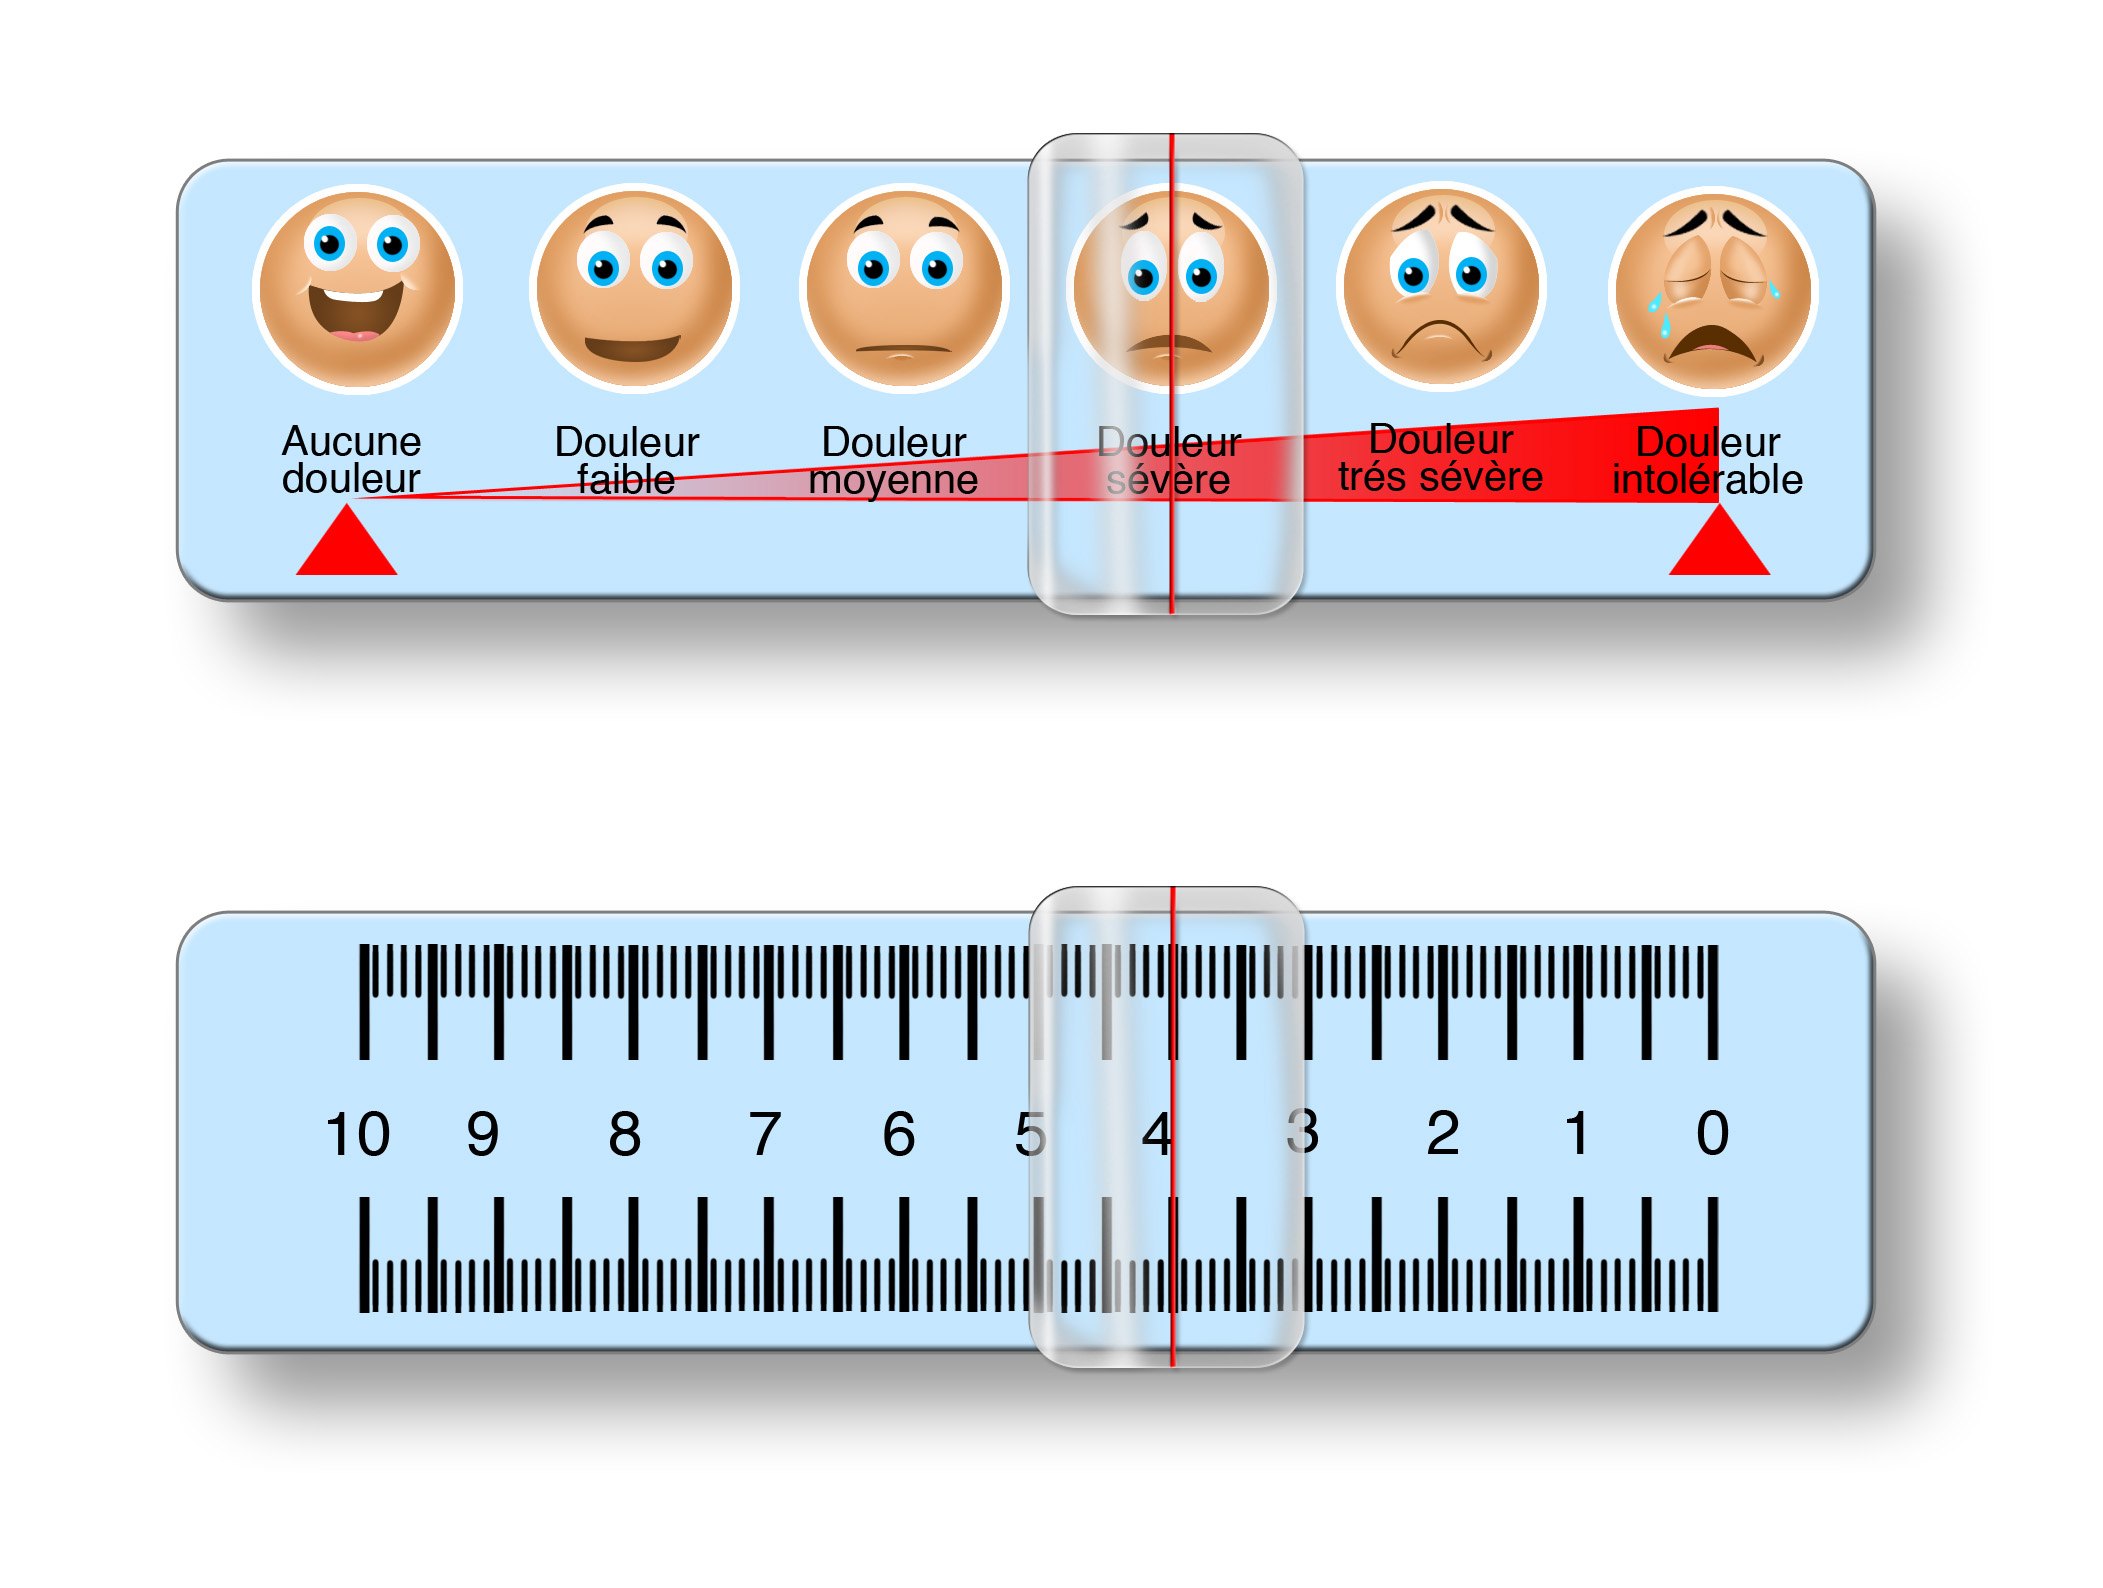
\includegraphics[height=.8\textheight]{fig/echelle-douleur.jpg}
\end{center}
\end{frame}

\begin{frame}{Organisation de la mémoire d'un ordinateur}
\begin{itemize}
\item Elle peut être vue comme un tableau d'octets avec :
\begin{itemize}
\item en \textit{indice} : le numéro de la case mémoire (commençant à 0) appelée l'\textbf{adresse}
\item en \textit{valeur} : la valeur de l'octet de la case mémoire référencée par l'indice
\end{itemize}
\end{itemize}
\begin{center}
\begin{tabular}{|l|l|}
\hline \textbf{adresse} & \textbf{valeur} \\
\hline 0 & ? \\
1 & ? \\
... & \\
234532 & 244 \\
... & \\
$n-1$ & \\
\hline
\end{tabular}
\end{center}
\end{frame}

\begin{frame}[fragile]
\frametitle{Déclaration d'une variable locale}
\begin{itemize}
\item Que se passe-t-il lorsqu'on déclare une variable ?
\begin{lstlisting}
char x = 'a';
\end{lstlisting}
\item Le système réserve une place en mémoire qui contient la valeur de \texttt{x}
\begin{itemize}
\item Il trouve une place libre (par exemple 22222)
\item dans la case associée, il stocke la valeur de la variable (ici \texttt{'a'})
\end{itemize}
\end{itemize}
\begin{center}
\begin{tabular}{|l|l|}
\hline \textbf{adresse} & \textbf{valeur} \\
\hline 0 & ? \\
1 & ? \\
... & \\
22222 & \texttt{'a'} \\
... & \\
$n-1$ & \\
\hline
\end{tabular}
\end{center}
\end{frame}

\begin{frame}[fragile]
\frametitle{Adresse d'une variable}
\begin{itemize}
\item En C(++), on peut demander l'adresse d'une variable : il suffit de préfixer son nom avec \&
%\begin{lstlisting}
%&x
%\end{lstlisting}
\item \texttt{\&x} représente l'adresse de \texttt{x}, c'est-à-dire 22222
\item Les adresses sont de simples entiers, mais C(++) permet de les typer par sécurité
\item Pointeur sur le type \textit{t} = adresse d'une variable de type \textit{t}
\item Exemples
\begin{itemize}
\item pointeur sur un entier : \texttt{int *}
\item pointeur sur un caractère : \texttt{char *}
\end{itemize}
\end{itemize}
\begin{lstlisting}
char *ptrX;
ptrX = &x;
\end{lstlisting}
\end{frame}

\begin{frame}[fragile]
\frametitle{Déréférencement}
\begin{itemize}
\item Déréférencement : accéder à la case mémoire \textit{pointée} par une adresse \texttt{t}
\item notation : \texttt{*t}
\end{itemize}
\begin{lstlisting}
cout << x << endl;
cout << *ptrX << endl;
\end{lstlisting}
\pause\begin{exampleblock}{Jouons un peu : qu'affiche ce bout de code ?}
\begin{lstlisting}
int a = 123;
int *x = &a;
*x = 342;
cout << a << endl;
cout << *x << endl;
\end{lstlisting}
\end{exampleblock}
\pause\begin{block}{Réponse}
342 \\
342
\end{block}
\end{frame}


% application des pointeurs

\begin{frame}[fragile]
\frametitle{Application des pointeurs : modifications des paramètres d'une fonction}
\begin{itemize}
\item Exemple d'une fonction qu'on ne sait pas écrire sans pointeurs : échange de deux variables
\item Passage par adresse (par opposition au passage par valeur)
\end{itemize}
\begin{lstlisting}
void echange(int *a,int *b) {
  int c = *a;
  *a = *b;
  *b = c;
}

// appel
int x = 124;
int y = 653;
echange(&x,&y);
cout << x << "," << y << endl;
\end{lstlisting}

\end{frame}

\begin{frame}[fragile]
\frametitle{Application des pointeurs : fonction retournant plusieurs valeurs}
\begin{lstlisting}
void sommediff(int a,int b,int *somme,int *diff) {
  *somme = a+b;
  *diff = a-b;
}

// appel
int s,d;
sommediff(23,18,&s,&d);
cout << s << "," << d << endl;
\end{lstlisting}

\end{frame}

% passage par adresse
\begin{frame}{Passage par adresse}
\begin{itemize}
\item Passer un paramètre à une fonction consiste à ce que la fonction reçoive \textbf{une copie} du paramètre dans une variable (qui porte le même nom ou pas)
\item Conséquence : si on modifie la copie, l'original n'est pas affecté
\item Que se passe-t-il si le paramètre est un pointeur ?
\begin{itemize}
\item Une \textbf{copie du pointeur} est fournie à la fonction appelée
\item La valeur de la copie (l'adresse) pointée ne sera jamais modifiée
\item Mais le contenu peut l'être par déréférencement
\end{itemize}
\end{itemize}
\end{frame}

\begin{frame}[fragile]
\frametitle{Rappel : pointeurs et structures de données}
\begin{itemize}
\item Si on a un type $A$ défini par \texttt{struct} ou \texttt{class}, un pointeur se définit par \texttt{A* ptr}
\item Comment accéder à un attribut \texttt{attr} de $A$ associé à \texttt{ptr} ?
\begin{itemize}
\item Logiquement : \texttt{(*ptr).attr} (attention aux priorités)
\item Raccourci : C(++) fournit une notation plus simple : \texttt{ptr->attr}
\end{itemize}
\item Attention : si le pointeur n'est pas initialisé, le déréférencement est une activité risquée...
\end{itemize}
\begin{exampleblock}{Exemple}
\begin{lstlisting}[language=C++]
int x;
int *y;
int z=*y;
\end{lstlisting}
\end{exampleblock}
\end{frame}

\subsubsection{Allocation dynamique de mémoire}

\begin{frame}[fragile]
\frametitle{Allocation mémoire en C}
\begin{itemize}
\item Allocation dynamique : réserver de la mémoire pendant l'exécution du programme
\item Réservation de mémoire avec \texttt{malloc}
\begin{lstlisting}
#include <stdio.h>
...
int *a = malloc(sizeof(int)));
struct machin *b = malloc(sizeof(struct machin));
// tableau
int *c = malloc(10*sizeof(int));
c[0] = 1; c[1] = 3;
\end{lstlisting}
\item l'opérateur \texttt{sizeof()} permet de connaître la taille d'une structure de données
\item Libération avec \texttt{free}
\begin{lstlisting}
free(a);
free(b);
free(c);
\end{lstlisting}
\end{itemize}
\end{frame}

\begin{frame}{Remarques}
\begin{itemize}
\item Penser à bien utiliser \texttt{sizeof()}, la taille des structures dépend de l'environnement d'exécution
\item De fait \texttt{malloc} et \texttt{free} ne sont pas typés et fonctionnent avec des \texttt{void *}
\item Ce sont de simples fonctions standard, on peut en utiliser d'autres (API Win32 par exemple)
\item Paradigme de gestion explicite de la mémoire : libérer tout ce qu'on alloue, par opposition au système de \textit{garbage collecting} à la Java
\item Mémoire pas initialisée + opérateurs pas typés + gestion explicite de la mémoire + accès tableaux pas vérifiés = une proportion significative de plantage des programmes C
\end{itemize}
\end{frame}

\begin{frame}[fragile]
\frametitle{Allocation mémoire en C++}
\begin{itemize}
\item Cela ne va pas résoudre tous les problèmes !
\item Réservation de mémoire avec l'opérateur \texttt{new}
\begin{lstlisting}
int *a = new int;
machin *b = new machin;
int *c = new int[10];
\end{lstlisting}
\item Plus besoin de spécifier la taille, plus de problème de type
\item Libération de la mémoire
\begin{lstlisting}
delete a;
delete b;
delete[] c;
\end{lstlisting}
\item Attention, il y a un piège !
\end{itemize}
\end{frame}

\begin{frame}[fragile]
\frametitle{Tableaux et pointeurs}
\begin{itemize}
\item Notion d'arithmétique de pointeurs...
\begin{lstlisting}
void f1() {
    int *a = new int[10];
    int *b = a;
    int i=0;
    while (i<9) {
        *b = i;
        b++; i++;
    }
    *b = i;

    for (int j=0 ; j<10 ; j++) {
        cout << "a[" << j << "] = " << a[j] << endl;
    }

    delete[] a;
}
\end{lstlisting}
\item On peut appliquer additions et soustractions aux pointeurs
\begin{itemize}
\item l'unité est la taille du type de l'élément pointé
\item utile pour parcourir vite des tableaux, mais dangereux à souhait
\item aucune vérification de validité n'est effectuée...
\end{itemize}
\end{itemize}
\end{frame}
% arithmetique de pointeurs

% effets de bord
\begin{frame}{Exercice}
\begin{itemize}
\item Écrire un petit bout de code qui parcourt un tableau avec des pointeurs en dépassant la taille du tableau
\item Que se passe-t-il
\begin{itemize}
\item s'il n'y a rien d'autre dans la fonction ?
\item si juste après la déclaration du tableau, d'autres variables sont déclarées ?
\end{itemize}
\item La réponse dépend du compilateur...
\end{itemize}
\end{frame}
% le pointeur void * et les conversions de type

\begin{frame}[fragile]
\frametitle{Le pointeur void *}
\begin{itemize}
\item On a vu que certaines fonctions retournaient un type \texttt{void *}
\item \textit{void} en anglais signifie "rien, nul", voir fonction qui ne retourne rien
\item Que signifie alors \texttt{void *} ? juste une adresse en mémoire, non typée
\item Attention : c'est un format d'échange de tout vers n'importe quoi...
\begin{lstlisting}
    int a[10];
    float *b;

    b = (float *)((void *) a);
\end{lstlisting}
\end{itemize}
\end{frame}
% lien entre pointeurs et tableaux

% un bout sur les smart pointers ?




\section{Bibliographie sommaire}

\begin{frame}{Bibliographie}
\begin{itemize}
\item B. Stroustrup (2013). The C++ programming Language, 4th edition. Addison Wesley.
\end{itemize}
\end{frame}

\begin{frame}{Cours en ligne}
\begin{itemize}
\item OpenClassrooms \url{http://fr.openclassrooms.com/informatique/cours/programmez-avec-le-langage-c}
\item cplusplus.com \url{http://www.cplusplus.com/doc/tutorial/}
\end{itemize}
\end{frame}
\end{document}
